

\title{Exploring Endofunctions via Composition}
%\author{
%        Chad Brewbaker \\
%        DataCulture LLC\\
%        Clive, Iowa 50325, \underline{U.S.A}
%}
\date{\today}

\documentclass{article}
\usepackage{listings}
\lstnewenvironment{code}{\lstset{language=Haskell,basicstyle=\small}}{}
\usepackage{minted}
\usepackage{hyperref}
\usepackage{amsthm}
\usepackage{graphicx}
\graphicspath{ {img/} }

\newtheorem{thm}{Theorem}[section]
\newtheorem{defn}[thm]{Definition}
\newtheorem{exam}[thm]{Example}
%\theoremstyle{plain}
%\newtheorem{thm}{Theorem}% reset theorem numbering for each chapter

%\theoremstyle{definition}
%\newtheorem{defn}[thm]{Definition} % definition numbers are dependent on theorem numbers
%\newtheorem{exmp}[thm]{Example}



\begin{document}

\maketitle

\begin{abstract}
We examine sets of functions $f(a)\rightarrow a$ on a finite set by chasing them under self-composition (iteration). Using this technique we derive an optimal subroutine for the brute force kernel of Babai's graph isomorphism algorithm. We also gain insight into the complexity of boolean matrix multiplication, AKS class primality tests, and integer factorization.
\end{abstract}

\section{Introduction}

In this paper we study sets of functions $f$ from a finite set $a$ back into $a$, $f(a) \rightarrow a$. In addition to mathematical notation we will also use the formal programming language Haskell \cite{hudak2007}.
\begin{code}
f :: a -> a 
\end{code}
% Alternatively, \inputminted{Haskell}{Program.hs}

The number of functions from a size $y$ set to a size $x$ set is $x^{y}$. In Haskell notation we write the type signature of such a mapping as

\begin{code}
f :: x -> y 
\end{code}

This duality between exponentials and functions gives a translation between algebraic and functional viewpoints.

It is no coincidence that John Atanasoff, inventor of the first electronic digital computer, had an early curiosity with exponents and logarithms, \cite{boyanov2003}.

Recall this algebraic identity we learned in primary school.

$$(a^{m})^{n} = a^{mn}$$

Translated from exponential notation into functional notation we have:
\begin{code}
curry :: n -> m -> a
curry' :: (n,m) -> a
\end{code}
We name these functions "curry" in reference to Haskell Curry \cite{curry1934}. Curry's rule states we can refactor between a function between passing multiple arguments, and a function that passes a tuple of values.

For endofuctions with two arguments $f(A,A)\rightarrow A$, Author Cayley \cite{cayley1851} noted we can abstract them into multiplication tables. Applying Curry's rule we can bind the first argument in the multiplication resulting in an endofuction with one argument.
\begin{code}
f :: (a,a) -> a
g :: a -> a -> a
h :: a -> (a -> a)
\end{code}

% I can never remember how to format umlauts etc in latex, http://tex.stackexchange.com/questions/57743/how-to-write-�-and-other-umlauts-and-accented-letters-in-bibliography (Chad)

J. Richard B\"{u}chi \cite{buchi1962} further described how we can use either transition (multiplication) tables, transition graphs, or transition trees to give us a viewpoint that best fits a discussion on two variable endofunctions. A quality English translation was made by Sylvia B\"{u}chi, Peter Deussen and Dirk Siefkes \cite{maclane1990}.

\begin{figure}[h]
    \centering
    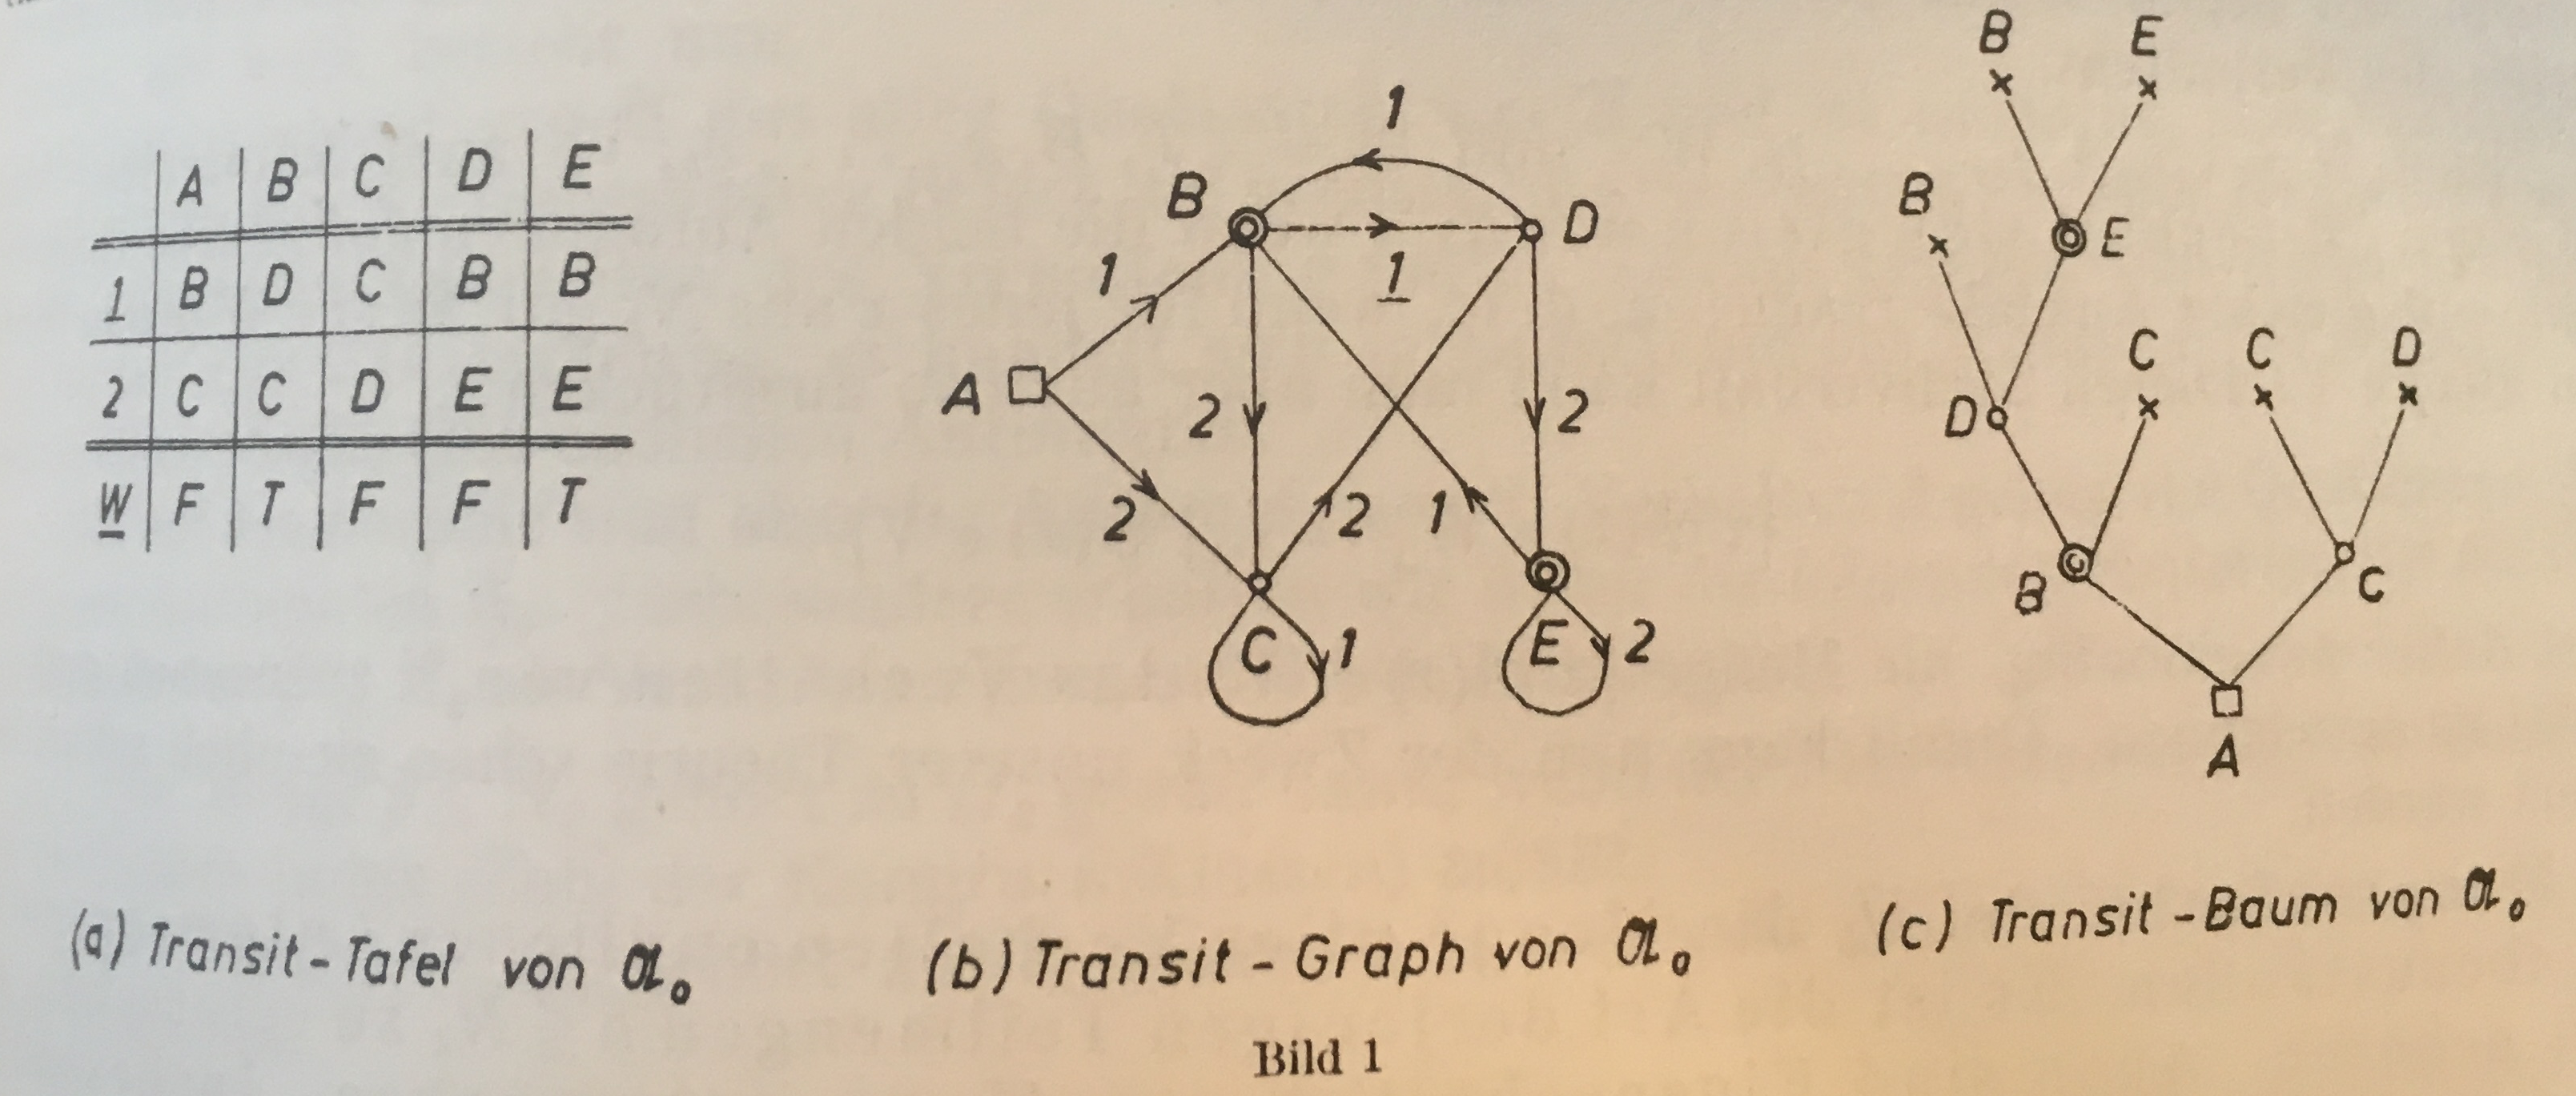
\includegraphics[height=4cm]{buchiTrinity}
    \caption{Diagram made by B\"{u}chi}
   
\end{figure}


\cite{alon1985} showed applications of endofuction composition for optimizing network transfers.

Here are definitions that are used.

%Extend our results to M{n} full set of full Magmas on $n$ elements? What crazy stuff happens? All the full mult tables on $n$ elements that are not associative plus $T_{n}$.
%Magma elements still have index and period. Only our results that require associativity will break.

%Automata (rows have labels of a different type than the column labels or entries) vs binary endofunctions.

%Given a multiplication tablediscuss how to test for totality O(n^2) make sure every entry is in bounds, asssociativity, identiy O(n) look at identity row/column, divisibility, and communitivy.

\begin{defn}[Endofunction] A function with domain and co-domain of the same type.\end{defn}
\begin{defn}[Semigroup] A collection of endofunctions closed under composition. Each endofunction may be thought of as a row in it's multiplication table. \end{defn}
\begin{defn}[Full Transformation Semigroup on $n$ elements ] The collection of all endofunctions on an $n$ element set. Denoted $T_{n}.$\end{defn}

\begin{exam} Multiplication table of $T_{2}$ here.\end{exam}

\begin{defn}[Iteration] Self composition of an endofunction. For $i$ self compositions on endofunction $f$ we denote this $f^{i}$\end{defn}

\begin{defn}[Index] Given an endofunction, the number iterations until it enters a cycle.\end{defn}
\begin{defn}[Period] Given an endofunction, the length of it's cycle under iteration.\end{defn}

\begin{defn}[Permutation] An endofunction with index of zero.\end{defn}

\begin{defn}[Symmetric group on $n$ elements] The set of all permutations on $n$ elements. Denoted $S_{n}$.\end{defn}
\begin{exam} Multiplication table of $S_{3}$ here.\end{exam}
\begin{defn}[Idempotent] An endofunction with index of zero and period of 1.\end{defn}

\begin{defn}[Reluctant function] An endofunction with index of at least 1.\end{defn}
\begin{defn}[Monogenic semigroup] A semigroup generated by one element. For permutations these are called cyclic groups.\end{defn}

\begin{defn}[Binary Matrix Multiplication] Matrix multiplication on the integers modulo 2. For this paper all matrices will be considered square.\end{defn}

\begin{exam} Multiplication table of $BMM_{2}$ here.\end{exam}

\begin{defn}[co-BMM] Matrix multiplication on the integers modulo 2 with addition an multiplication operations swapped.\end{defn}

\begin{defn}[$Z^{+}_{n}$] Integers modulo $n$ under addition. \end{defn} 

\begin{exam} Multiplication table of $Z^{+}_{6}$ here.\end{exam}

\begin{defn}[$Z^{\times}_{n}$] Integers modulo $n$ under multiplication. \end{defn} 

\begin{exam} Multiplication table of $Z^{\times}_{6}$ here.\end{exam}

\begin{tabular}{ |c |c |c |c |c |c |c | }\hline
$Z_6^\times$&0&1&2&3&4&5\\ \hline
0&0&0&0&0&0&0\\ \hline
1&0&1&2&3&4&5\\ \hline
2&0&2&4&0&2&4\\ \hline
3&0&3&0&3&0&3\\ \hline
4&0&4&2&0&4&2\\ \hline
5&0&5&4&3&2&1\\ \hline
\end{tabular}

\begin{defn}[Factoring] Given an endofunction $f$; return two endofunctions $g,h$, neither an identity function, such that $ f = g(h)$.\end{defn}
\begin{defn}[Multiplication] Given an endofunctions $g,h$; return an endofuction $f$, such that $ f = g(h)$.\end{defn}
\begin{defn}[Left factoring] Given an endofunctions $f,h$; return an endofuction $g$, such that $ f = g(h)$.\end{defn}
\begin{defn}[Right factoring] Given an endofunctions $f,g$; return an endofuction $h$, such that $ f = g(h)$.\end{defn}



\begin{defn}[Game of Life] Automata on orthogonal grid with binary values defined by John Conway. For this paper we will use square toroidal grids, Top/Bottom rows and Left/Right columns are considered adjacent. 
States are Live and Dead. Live cell with less than two Live neighbors dies. Live cell with 2 or 3 Live neighbors lives.  Live cell with more than 3 Live neighbors dies. Dead cell with exactly 3 live neighbors becomes Live.\end{defn} 

\begin{defn}[Detection] Given two endofunctions $f$ and $g$, if $f^{i} = g$, then $g$ is said to detect $f$. \end{defn}


\begin{exam} Examples with permutations and $Z_{1000}^{\times}$\end{exam}


Our first tool is "endoscope". It is a function on an ordered set $a$. The arguments are a list of elements in the set $a$, and the endofunction under study. It returns pairs of element in the set and where it ends up after some number of self-compositions.
\begin{code}
endoscope :: Ord a => [a] -> (a -> a -> a) -> Set (a,a)
\end{code}


The function "idempotents" takes a list of elements and an endofunction. It returns the list of elements that are idempotent when passed through the endofunction.
\begin{code}
idempotents :: Ord a => [a] -> (a -> a -> a) -> [a]
idempotents elts mult = filter isSame elts 
       where
        isSame x = mult x x == x 
\end{code}



Crypto hash to  256 bits
Count


\section{Permutation function spaces, $S_{n}$}

\begin{code}
perm :: a -> a
-- perm must be a cycle under iteration 
\end{code}


Edges under iteration

Idempotents (connected components)

Histogram of index,period.

Forgetfull functions: By definition permutation function sets have no forgetfull functions.

Leaves

Group-likes
\section{Transformation function spaces, $T_{n}$}

Edges under iteration

Idempotents (connected components)

Histogram of index,period.

Reluctant functions. \cite{mullin1970} 

Leaves

Group-likes



\section{Multiplication in $Z_{n}$ }

Edges under iteration

Idempotents (connected components)

Histogram of index,period.

Reluctant functions

Leaves

Group-likes


What does this tell us about integer factorization?


\section{Addition in $Z_{n}$ }

Edges under iteration
\href{http://www.oeis.org/A057660}{OEIS A057660}, the sum of orders of elements in a cyclic group with $n$ elements. $$\sum_{k=1..n} {n \over GCD(n,k)}$$

Idempotents (connected components)

Histogram of index,period.

Reluctant functions

Leaves

Group-likes

\section{AKS Primality endofuction}
%In \cite{anderson2005}  proved that an iterated endofuction 

Borwein \cite{borwein1985} showed us that computing $n!$ by successive multiplications was rather inneficient.

$$8! =2*3*2^{2}*5*(2*3)*7*(2^{3})$$

Instead, we can take the table of all primes up to $n$, figure out how many times each prime factor is applied and exponentiate each prime factor once to the appropriate power.
$$8! = 2^{7}*3^{2}*5*7$$

Geotgheluck showed us how to compute binomial coefficients using prime factorizations, \cite{goetgheluck1987, goetgheluck1988}.


% Chad 
%Is Geotgheluck's method any faster than applying Borwein's to $n!, k!, (n-k)! $ then subtracting the denominator exponents?

AKS noted that for prime numbers ${n \choose k}$ always is divisible by  $n$, since no term in the denominator less than $n$ is a factor. ${n! \over k! * (n-k)!}$

However for composite numbers $n$ , some values of ${n \choose k}$ are not divisible by $n$.

\begin{code}
aksBinomial :: Integer -> Integer -> Integer
aksBinomial n k = mod (binomial n k) n
\end{code}

When this function returns a nonzero value, we know that $n$ is a composite number.

% $p(x)\equiv q(x)$ mod $(x^{r}-1 ,n)$ denotes both $p(x)\equiv q(x)$ mod $x^{r}-1$ and $p(x)\equiv q(x)$ mod $n$.

% Chad
% Can we use Borwein factorial simplification to cheat? Know that if $n$ is not prime then we don't need another entry into our prime table. $n$ will be a composite of others. With k= n-1 
% binomial n k = binomial (n-1) (k-1) +  binomial (n-1) k

%\prod_{i=1}^{k} {n +1 + i) \over i } \prod_{i=1}^{k} {n -(k -i)) \over i }


% If $k$ is  sqrt(n) +1 then either that bottom $k!$ whacks out a chuck, or it leaves that largest number unfactored.
%can we take successive $2^{i}!$ to find the order of magnitude of the smallest prime divisor?

\section{Boolean matrix multiplication }
Boolean ($Z_{2}$) matrix-matrix multiplication (BMM) is a fundamental subroutine. Computations from transitive closure to parsing context free grammars\cite{valiant1975} reduce to BMM.

Traditionally the complexity of BMM is written by $O(n^{\omega})$, where $\omega$ shrinks from the brute force value of $3$ as researchers since Strassen have derived more efficient BMM algorithms.

Endoscope groups matrices into connected components under self composition. 
%My personal conjecture is that BMM is $O((n log n)^{2} )$ (Chad)
% http://math.stanford.edu/~church/BCCGU-On-cap-sets-and-the-group-theoretic-approach-to-matrix-multiplication.pdf Note that the Umans conjecture for \omega=2 was just disproven.
% bmm :: m -> m -> m
% $m^{m \times m}$ is the function space where $m$ is a set the size $2^{m \times m}$
%Of course we aren't grabbing all functions from that pair, just those that are legal BMM results.
%Can we come up with a compression method formulation as a BMM lower bound?
%Compress the serialized m,m,m triples into FSA. Do FSA minimization. Feasible on 3x3 BMM? (2^{9})*(2^{9}) words in the language. All words length 27.
%What permutation of these triples allows us to reduce average rejection prefix for an illegal word? Thats feasible for 2x2 BMM very quickly.

Edges under iteration

Idempotents (connected components), same as fixed points?

Histogram of index,period.

Forgetfull functions

Leaves

Group-likes


What does this tell us about the complexity of BMM?



\section{Boolean matrix co-multiplication }
We define boolean matrix-matrix co-multiply (co-BMM) as the function where we have swapped the multiply and addition operators. 

As a data type, each resulting entry is the $n$-tuple consisting of entries that are either $A_{i,k}$ or $B_{k,j}$. If view $A$ and $B$ as graphs, with rows being outgoing edges and columns as incoming edges; we have $n$-tuples of chosing either the incoming or outgoing edge for each entry.


Edges under iteration

Idempotents (connected components), same as fixed points?

Histogram of index,period.

Forgetful functions

Leaves

Group-likes


What does this tell us about the complexity of co-BMM?

\section{Transformation polynomials }
In \cite{ashlock1990} the concept of a permutation polynomial over $Z_{n}$ was studied. These are polynomials with coefficients and powers from $Z_{n}$ that form a permutation function on $Z_{n}$. We extend this concept to all polynomials with coefficients and powers from $Z_{n}$. Interestingly, transformation polynomials seem to form a generalization of the AKS style primality test as prime numbers and composite numbers have form radically different sets of transformations.

Edges under iteration

Idempotents (connected components), same as fixed points?

Histogram of index,period.

Reluctant functions

Leaves

Group-likes


What does this tell us about the complexity of co-BMM?


\section{Compositional equality relations}

\appendix{New OEIS Sequences}

\appendix{Haskell source}

\nocite{*}
\bibliographystyle{plain}
\bibliography{biblio}
\end{document}
